% DISCUSSION CONTENT

\section{Impact of this work}
In this work, we made scientific contributions to the field of computational biology applied to single-cell omics. More specifically, we developed approaches for performing trajectory inference and network inference analyses for single-cell omics, as well as approaches for assessing the performance of such methods in a quantitative way.

The contribution with the largest impact in the field is the large-scale comparison of 45 TI methods. Based on our results, we provided guidelines on how to perform a TI analysis and developed a toolkit for performing a inferring and interpreting trajectories using any of these methods. Since such guidelines were hitherto lacking, they are now commonly disseminated in manuscripts \cite{lafzi_tutorialguidelinesexperimental_2018, luecken_currentbestpractices_2019}, courses \cite{kiselev_analysissinglecell_2019, martens_analysissinglecell_2019}, and slides shown during keynote caffeine refuelling sessions \cite{hemberg_coffeebreakanalysis_2019}. These disseminations are having a significant impact in how TI analyses are being performed in academia and industry alike.

This dissertation commences with a rant on low self-assessment rates of method developers. As a result, we developed a simulator of \textit{in silico} single cells, that allow quantifying the accuracy the prediction of a tool, even if the real data required to perform this analysis does not exist yet. While the manuscript is not published yet, dyngen has already been used to evaluate trajectory inference \cite{saelens_comparisonsinglecelltrajectory_2019}, trajectory-based differential expression \cite{vandenberge_trajectorybaseddifferentialexpression_2019}, and network inference \cite{pratapa_benchmarkingalgorithmsgene_2019} methods. 


% has used dyno detomaso_functionalinterpretationsingle_2019

\section{Outlook}
The types of computational analyses presented in Section~\ref{sec:comptools} (Clustering, DE, DR, TI, NI) all become routine methodologies for analysing and interpreting single-cell omics data. Here, we discuss several promising categories of computational methods that are currently still in a exploratory stage (Figure~\ref{fig:scapplications_extended}).


\begin{figure}[htb!]
	\centering
	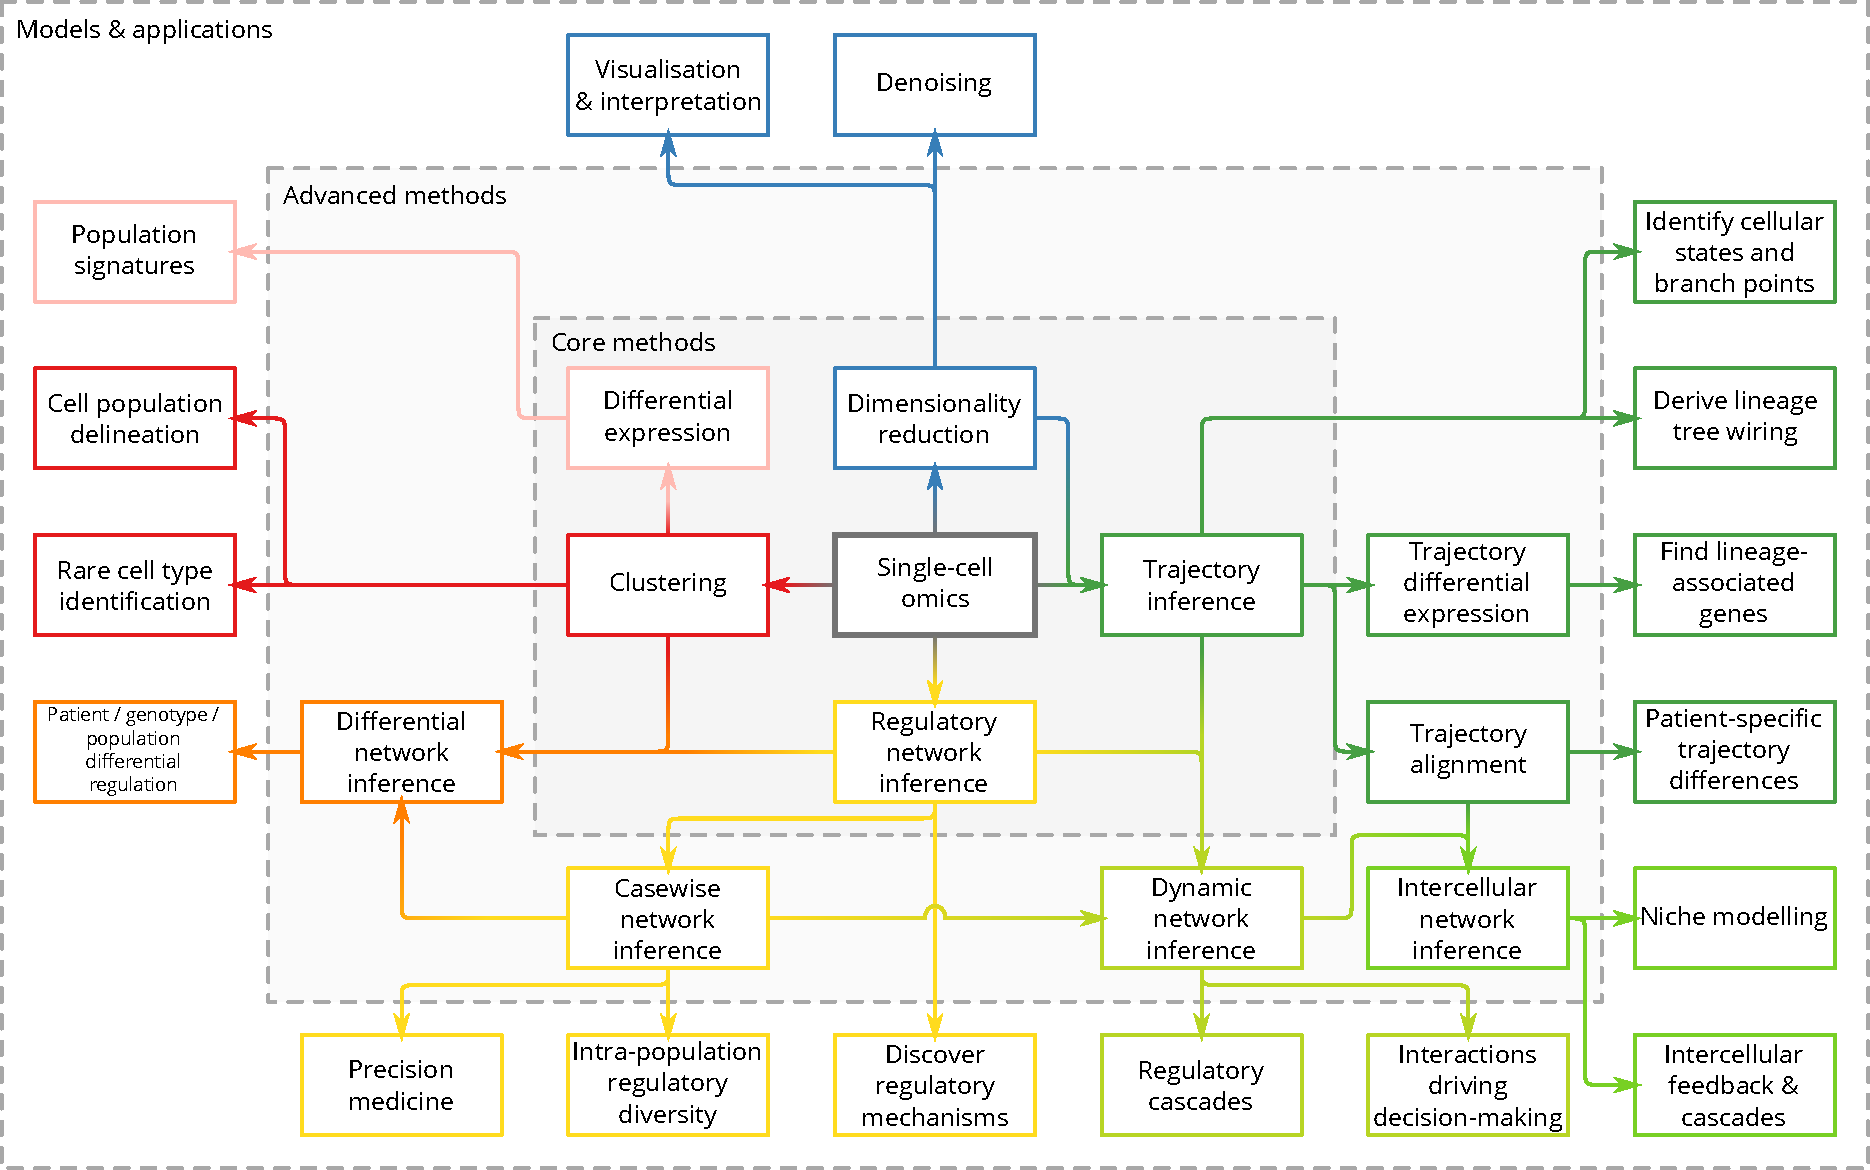
\includegraphics[width=\linewidth]{fig/singlecell_technologies_v8.pdf}
	\caption{Developments in computational methods for single-cell omics. Adapted from presentations by Wouter Saelens and myself.}
	\label{fig:scapplications_extended}
\end{figure}


\subsection{Trajectory differential expression}
Trajectory inference methods have made transformative changes in single-cell omics by allowing to study how cells change during a dynamic process of interest in a high-throughput and unsupervised approach. 
A crucial aspect in analysing and interpreting the resulting trajectories is the discovery of genes whose expression significantly shifts in a region of interest within the trajectory, called Trajectory Differential Expression (TDE).

Several trajectory inference methods offer TDE functionality as part of downstream analysis and interpretation of the outputted trajectories \cite{cannoodt_scorpiusimprovestrajectory_2016,qiu_reversedgraphembedding_2017,lonnberg_singlecellrnaseqcomputational_2017,wolf_pagagraphabstraction_2019}. However, current approaches typically cluster cells and perform differential expression analyses between the clusters, or are otherwise limited towards detecting differential expression of a gene along linearly ordered cells along one lineage path in the trajectory.

tradeSeq \cite{vandenberge_trajectorybaseddifferentialexpression_2019} is a generalised TDE method which can be used to discover different types of differential expression along a trajectory, which can be applied as a downstream analysis to trajectories inferred from any TI method. By including a comparative benchmark of TDE methods on real and synthetic data, Van den Berge et al. started a rational dialogue on TDE methodology.

\subsection{Trajectory alignment}
Trajectory alignment allows studying the differences between multiple trajectories that are mostly similar. For example, the cell developmental process of a patient could be compared to that of a healthy control to detect the transcriptomic differences of a particular lineage branch. 

Trajectory alignment has been used to compare gene expression kinetics resulting from different biological processes\cite{cacchiarelli_aligningsinglecelldevelopmental_2018}, to compare human, chimpanzee and macaque neuronal development\cite{kanton_organoidsinglecellgenomic_2019}, to find differences in gene regulation in the presence of certain growth factors\cite{mcfaline-figueroa_pooledsinglecellgenetic_2019}, and to compare human and mouse embryogenesis\cite{alpert_alignmentsinglecelltrajectories_2018}.

However, aligning trajectories becomes exponentially more difficult as the complexity of compared trajectories increases. For this reason, trajectory alignment remains a mostly unexplored territory within single-cell omics.

Dynamic Time Warping (DTW) \cite{giorgino_computingvisualizingdynamic_2009} is most commonly used to align linear trajectories. DTW is a technique originating in the field of speech recognition and aligns temporal sequences by creating a warping path between two sequences that indicates which sequence must be dilated or contracted to best match the other one.

Over time, as the affordability of single-cell omics technologies improves and the abundance of available datasets increases, we hypothesize that these methods will become highly relevant in comparing dynamic processes in samples from multiple donors.

\subsection{Differential network inference}
Differential NI methods aim to reconstruct one network for each of the given conditions amongst the transcriptomic profiles. The conditions can be different cellular states or changes in environment, and profiles can be grouped according to prior knowledge or derived through unsupervised clustering. From the resulting networks, one can then investigate the pathways that are differentially activated between conditions (e.g. deregulated pathways between a diseased and healthy condition), or those that are similarly activated between conditions (e.g. similarly activated pathways between two different disease conditions).

Differential NI methods have already been described for bulk -omics data \cite{Ideker2012}, where they have been used, for instance, to elucidate deregulated mechanisms in different subtypes of leukaemia \cite{Gill2014}.

\subsection{Dynamic network inference}
Advances in single-cell transcriptomics have fostered the development of trajectory inference methods \cite{Cannoodt2016}, which are computational tools to reconstruct dynamic processes such as cellular differentiation and cell cycle (Figure \ref{fig:ti_with_ni}). These methods usually recover the underlying structure of the data by focusing on the similarities between cells. The cells can then be ordered along a trajectory that optimally models the data structure.  
This bears resemblance to the more traditional time-series experiments with bulk transcriptomics data, albeit at a much higher temporal resolution. Unlike time-series experiments, trajectories are ideally inferred in an unsupervised manner, as not to introduce human bias.

As in time-series experiments, NI methods can exploit the information provided by trajectory inference methods in order to improve the resulting regulatory network. Several NI methods use this information in order to determine the directionality and the type of an interaction. This has helped to construct more accurate boolean networks (SCNS \cite{Moignard2015}), by selecting the network that most reliably describes the observed cell ordering. Several NI methods use this cell-ordering information to construct ordinary differential equations that are again improved to optimally describe the observed data \cite{Ocone2015,Wei2016}. While such methods are generally able to improve the accuracy of the produced networks by using information from the trajectory, they suffer from the same limitations as discussed at the start of the section since they produce a single regulatory network that is supposed to be a model for all of the cells in the population.

Instead, dynamic NI methods produce a network of interactions with variable activation levels across the trajectory. They provide useful information on which transcription factors are expressed at the beginning of a developmental process, and which gene interactions occur at later stages for instance. Dynamic networks are more complex models in comparison to differential and static networks. 


\subsection{Casewise network inference}
Casewise network inference (CNI)
methods\footnote{Other terms are commonly used when dealing with data from a particular source. For example, single-cell NI when applied to single-cell transcriptomics data; sample-specific NI when applied to bulk transcriptomics; patient-derived NI when applied to bulk profiles of patients.}
predict not only which transcription factors regulate which target genes
(Figure~\ref{fig:scgrn}A, top left), but also how active each
interaction is in every case (Figure~\ref{fig:scgrn}A). In CNI, a `case'
might be a cell, but it might also refer to a bulk sample.

While a few pioneering CNI approaches have already been
developed\autocites{aibar_scenicsinglecellregulatory_2017}{kuijjer_estimatingsamplespecificregulatory_2019}{liu_personalizedcharacterizationdiseases_2016},
a quantitative assessment of the performance is hitherto lacking. This
is not surprising, as neither real nor in silico datasets of
cell-specific or even cell-type-specific interactions exists that is
large enough so that it can be used as a ground-truth for evaluating CNI
methods.

\subsection{Intercellular network inference}
Cells are influenced by extracellular signals produced by cells
in their microenvironment. One way of studying intercellular
communication is to profile gene expression in interacting cells.
Especially single-cell-omics technologies are promising because
of their ability to analyze tissue composition in high resolution \cite{yosef_writlargegenomic_2016,tanay_scalingsinglecellgenomics_2017} .
Furthermore, spatial and sophisticated single-cell transcriptomics
technologies have recently been developed to assay the spatial con-
text of a cell \cite{stahl_visualizationanalysisgene_2016,rodriques_slideseqscalabletechnology_2019,eng_transcriptomescalesuperresolvedimaging_2019,vickovic_highdefinitionspatialtranscriptomics_2019} , characterize cellular niches 7 or construct physical
cell–cell interaction maps 8 .
Several studies have recently demonstrated the potential of
single-cell transcriptomics to investigate intercellular communica-
tion 9–14 . There, computational methods, such as CellPhoneDB 14 ,
were applied to infer links between ligands (that is, extracellular
protein signals) expressed by sender cells and receptors expressed
by receiver cells. Thus, these computational approaches elucidate
by which extracellular signals cells can communicate. Nevertheless,
a functional understanding of cell–cell communication requires
knowledge about the influence of these ligand–receptor interac-
tions on target gene expression. Hence, there is a need for compu-
tational methodologies that use expression data of interacting cells
to infer the effects of sender-cell ligands on receiver-cell expression.
Although a few basic methods were developed for bulk data (for
example, CCCExplorer) 15,16 , comprehensive and predictive methods
that are generally applicable to both bulk and single-cell expression
data are lacking.


% When does a cluster represent a new cell type? \cite{kiselev_challengesunsupervisedclustering_2019}



\section{A life without Git, Travis CI, or tidyverse}
A significant portion of this work involved developing large software libraries, in a collaborative setting, over a time span of about four years. Since the results of our comparison of 45 TI methods required three years to develop, we were happily forced to develop a system where experiments could be rerun and results could be updated on-the-fly.

We summarised our experiences in the form of a set of guidelines for benchmarking computational tools (Chapter~\ref{chap:guidelines}). However, these guidelines do not touch upon many aspects of good software development practices that we learned to use in order to bring this thesis to a good end. In particular, I would like to highlight several  fundamental (open-source) projects without the likes of which our research would have been simply impossible to perform, namely Git, Travis CI, and the tidyverse.

\textbf{Git} \cite{torvalds_gitfastversion_2005} is a code-revision system that allows multiple users to collaborate on developing code and keep track of what changes were made by whom. 
Since Wouter Saelens and I were often working closely together on a specific part of our software, Git saved us a lot of time by merging together changes developed in parallel. Only in few cases did we need to intervene manually to merge our changes.
Additionally, Github.com allowed us not only to collaborate with each-other, but also correspond and collaborate with other software developers from many different research groups, using Github Issues to discuss problems with other researchers, and Github Pull Requests to contribute code to open-source projects. 

Together, we published over 20'000 code contributions (commits) across 50+ software packages \cite{cannoodt_developmentdynverse_2019}. Since many of these packages depend on one another, it is inevitable that changes made to one package would break another package. We wrote many, many unit tests (and still too few), and we let these tests automatically be executed on \textbf{Travis CI} \cite{traviscigmbh_traviscitest_2011}. This way, when we pushed breaking changes to Github, Travis CI would notify that our commit has resulted in one or more unit tests failing. While sometimes it is a hassle to set up, Travis CI has prevented us countless times from generating faulty results due to a faulty underlying function.

Software bugs can be introduced even by incredibly small, seemingly insignificant changes. The R programming language seems particularly susceptible towards getting trapped by its many pitfalls. However, there are many benefits of using R in bioinformatics research context, such as its extensive community of statisticians develop packages for the R ecosystem. The \textbf{tidyverse} packages \cite{wickham_welcometidyverse_2019}, developed by the RStudio team and many online contributors, completely transformed my experiences with R from tedious struggles to efficient everyday functional programming.

Honourable mentions go to Linux, Fedora, \LaTeX, TeXstudio, (R)Markdown, Bash, Sed, Regular expressions, Rocket Chat, for making bioinformatics software development even more fun and enjoyable.

% ideas:
%  Yet I wonder how the current academic system
%can support such concepts. Academics often hold different positions in
%different research groups around the world, who should be the maintainer in
%these cases? The original PhD students that developed the work? The original
%research group?

%The eight chapter is a manuscript in preparation about the assessment of TI methods. The main discussion topic is the lack of a quantitative measure for the scoring of new TI methods. This leads to the publication and development of new methods that do not show a clear performance improvement compared to other methods. The main topic touches
%upon some sore points that are inherent in bioinformatics. The main thought I have with
%this chapter is that defining clear goals in an emerging technology is difficult and therefore is sometimes ignored by fellow bioinformaticians. This because the lack of standardized performance metrics, missing public datasets that are well described and an \textit{ad hoc} problem definition. I follow the idea of defining a clear cut approach to benchmarking (as described in chapter nine) and I like the proposition that is started in this manuscript for a discussion on good TI metrics.} Would approaches like e.g. DREAM challenges be a means of tackling these issues to your opinion?

% zie peter dawyndt, chapter 5
\clearpage
\section{References}
\printbibliography[heading=none]
